\chapter{Realisierung des FIR-Filters}\label{Cha:RealFIR}
\section{Aufgabenstellung}
Die Aufgabenstellung bestand darin, ein FIR - Mittelwertfilter zu realisieren und auf verschieden Weisen zu implementieren.
Anschließend wurden die Implementierungen auf ihre Leistung untersucht und verglichen. Es handelt sich jedes mal um ein FIR - Mittelwertfilter vierter Ordnung.

\section{Durchf\"uhrung}
Gemäss des Umdrucks wurde ein Projekt erstellt und die entsprechenden Dateien angefügt. In einem ersten Teil wurde dann die Sprungantwort mithilfe einer Simulation durch händisches verändern der Eingangswerte ermittelt und aufgenommen. 
In der folgenden Tabelle sind die von uns manipulierten Werte und die in sDAC1L resultierenden Werte aufgezeigt.
\begin{center}
\begin{tabular}{|c|c|}
\hline 
Eingang & Ausgang \\ 
\hline 
0 & 0 \\ 
\hline 
25716 & 5143 \\ 
\hline 
25716 & 10286 \\ 
\hline 
25716 & 15429 \\ 
\hline 
25716 & 20572 \\ 
\hline 
25716 & 25716 \\ 
\hline 
25716 & 25716 \\ 
\hline 
%%\caption{Erfassung der Sprungantwort\textunderscore Mode}
\end{tabular} 
\end{center}

Im nachfolgenden Bild ist diese Annäherung grafisch dargestellt. Man erkennt gut, dass sich der Ausgangswert sukzessive und linear dem Eingangswert annähert. 
Dies passiert in fünf Schritten, wie es für ein solches Filter üblich ist und entspricht damit den Erwartungen
\begin{figure}[H]
  \centering
    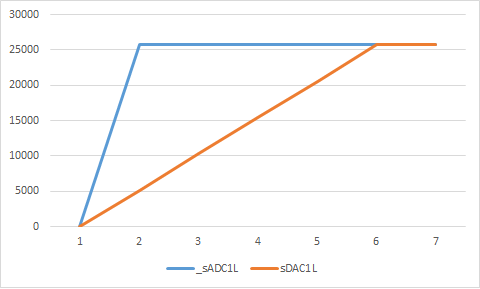
\includegraphics[width=\textwidth]{Sprungantwort1.png}
  \caption{Sprungantwort des FIR Filters\textunderscore Mode\textunderscore Sprungantwort1.png}
  \label{fig:SprAW1.png}%%Konvention figures immer mit fig:
\end{figure}
 %%%%%%%%%%%%%%%%%%%%%%%%vergleich mit vorbereitung
 In der Vorbereitung wurde die Sprungantwort eines Filters vierter Ordnung ermittelt, welche auf dem folgenden Bild zu sehen ist.
 %%%%%%%%%%bild SprungantwortMittelwert.png
 \begin{figure}[H]
  \centering
    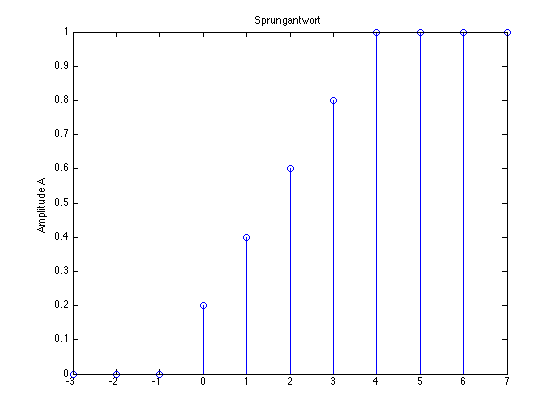
\includegraphics[width=\textwidth]{SprungantwortMittelwert.png}
  \caption{Sprungantwort des FIR Filters aus der Vorbereitung\textunderscore Mode\textunderscore SprungantwortMittelwert.png}
  \label{fig:SprAW.png}%%Konvention figures immer mit fig:
\end{figure}
 Trotz der Unterschiedlichen Darstellungsarten ist eindeutig zu sehen, dass sich die Filter gleich verhalten.
 
 Es wurde eine Programmzyklenzahl von 1672 ermittelt.
 
 Im nächsten Schritt wird diese Herangehensweise wiederholt, diesmal allerdings mit Zahlen im 1.15 Format. Dazu wurden die Variablen auf den Typ short Integer im C-Code angepasst.\\
 \begin{adjustbox}{width=\textwidth,height=\textheight,keepaspectratio}
 \begin{lstlisting}[title=fir.c]{fir.c}
#include "fir.h"

short fir(short sInput, FIRstate *pFIR) {

	int k;
//	float acc; //Datentyp gemaess Aufgabe angepasst
	int acc;
	
	*(pFIR->p++)=sInput;	// store current sample in delayline
	if ( pFIR->p >= pFIR->d + pFIR->N) pFIR->p-=pFIR->N;

	for (acc=0,k=0;k<pFIR->N;k++) {
		acc += (*(pFIR->p++) * pFIR->h[k]);
		if ( pFIR->p >= pFIR->d + pFIR->N) pFIR->p-=pFIR->N;
	}
	
	return (short)(acc >> 15); //rightshift um nur hoeherwertige Bits zu verwenden
}
\end{lstlisting}
\end{adjustbox}
Wie zu sehen ist wurden im Vergleich zur Ursprungsversion zwei Änderungen vorgenommen: acc wurde zu einem Integer und der Typecast im return-statement wurde um einen Rechtsshift erweitert. Die erste \"Anderung erklärt sich aus der Aufgabe da mit short Integer gerechnet werden sollte, wobei acc das ergebnis einer Multiplikation ist, welche so viele Bits hat wie beide Summanden zusammen, deshalb int statt short. Der Rechtsshift sorgt daf\"ur, dass nur die 15 h\"oherwertigen Bits zum short getypecastet werden.\\\par
Wir \"uberprüften die Funktionsweise wie oben und erhalten folgende 
Messwerte:\\
\begin{center}
\begin{tabular}{|c|c|}
\hline 
0 & 0 \\ 
\hline 
0,5 & 0,1 \\ 
\hline 
0,5 & 0,2 \\ 
\hline 
0,5 & 0,3 \\ 
\hline 
0,5 & 0,4 \\ 
\hline 
0,5 & 0,5 \\ 
\hline 
0,5 & 0,5 \\ 
\hline 
\end{tabular} 
\end{center}
woraus folgende Grafik entsteht.
\begin{figure}[H]
  \centering
    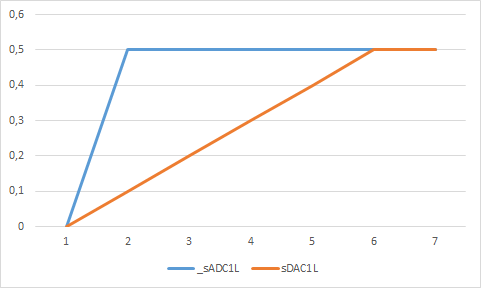
\includegraphics[width=\textwidth]{Sprungantwort2.png}
  \caption{Sprungantwort des FIR Filters im short Integer Format\textunderscore Mode\textunderscore Sprungantwort2.png}
  \label{fig:SprAW2.png}%%Konvention figures immer mit fig:
\end{figure}
Wieder sind alle Werte wie erwartet.
Die Messung ergab eine Programmzyklenzahl von 764, was eine deutliche Leistungsverbesserung gegen\"uber des Versuches zuvor ist, was sich darin begr\"undet, dass der DSP f\"ur 16-Bit-Operationen optimiert ist.\\
In einem weiteren Optimierungsschritt wird das Filter nun in Assembler umgesetzt um Optimierungen zu nutzen die der Compiler sonst nicht nutzt, wir erwarten eine schnellere Abarbeitung.
Dazu wurde die Datei fir.asm im Bereich f\"ur die Funktion \textunderscore fir: angepasst:
\begin{adjustbox}{width=\textwidth,height=\textheight,keepaspectratio}
 \begin{lstlisting}[title=fir.c]{fir.c}
//!! Begin of Setting I, L, and B regs	
B1 = P1; //Basis: Erstes Verzoegerungsglied, hier delay line.
R1 = R1 << 1; //Mal 2, weil Short Int 2 Byte hat.
L1 = R1; // Laenge festlegen auf 2 mal 2 Byte.
I1 = P2; // I1 auf Read/Write legen
I2 = P0; // I2 auf Filterkoeffizienten
//!! End of Setting I, L, and B regs

\end{lstlisting}
\end{adjustbox}
Die Register werden so konfiguriert, dass die Funktionalität des Filters abgebildet wird, vergleiche hierzu den kompletten Code siehe Anhang. I2 beinhaltet dabei die \"ubergebenen Filterkoeffizienten und wird mit I1 multipliziert, was den aktuell \"ubergebenen Werten entspricht. L1 ist die L\"ange des zyklischen Speichers und muss damit der Ordnung des Filters multipliziert mit dem Speicherbedarf eines Wertes, hier 2 Byte multipliziert werden. Der Anfang des Speichers muss logischer Weise der Anfang des Filters sein, hier Parameter P1.\\

Auf die Aufnahme einer Messreihe und der entsprechenden Grafik wird der Übersichtlichkeit halber ab hier verzichtet, da die Versuche gezeigt haben, dass die Messreihen jedes mal identisch aussehen, lediglich die Programmzyklenzahl hat sich verändert. Sie beträgt in diesem Fall 100, was einer weiteren Performanceverbesserung und unseren Erwartungen aus oben gegebenem Grund entspricht.\\
Der letzte Optimierungsschritt nutzt die Fähigkeit des DSPs zur parallelen Abarbeitung zweier MAC-Operationen aus. Dazu wurde die Funktion zum Aufruf der Filterfunktionalität wie in der Aufgabe beschrieben ersetzt, die isr.c zum Aufruf der Stereofunktion durch Auskommentieren verändert und fir.asm wie folgt angepasst. Im Teil \textunderscore fir\textunderscore stereo: wurden Register wie folgt angepasst.

\begin{adjustbox}{width=\textwidth,height=\textheight,keepaspectratio}
 \begin{lstlisting}[title=fir.c]{fir.c}
//!! Begin of Setting I, L, and B regs	
B1 = P1; //Basis: Erstes Verzoegerungsglied, hier delay line.
R1 = R1 << 2; // 4*R1 da 32 Bit -> 8Bit*4=32
L1 = R1; // Laenge festlegen auf 4 mal 2 Byte.
I1 = P2; // I1 auf Read/Write legen
I2 = P0; // I2 auf Filterkoeffizienten
//!! End of Setting I, L, and B regs
\end{lstlisting}
\end{adjustbox}
Diese Konfiguration entspricht der selben wie in der Aufgabe zuvor, mit dem Unterschied, dass der Speicher doppelt so lang ist. Dies begr\"undet sich darin, dass nun zwei Werte gleichzeitig bearbeitet werden.\\
Auch in diesem Fall wurde die Programmlaufzeit ermittelt und ist mit 52 Zyklen die schnellste, auch dies haben wir auf Grund der nun parallelen Abarbeitung erwartet.



\section{Auswertung}
Es soll die maximal m\"ogliche Anzahl an Ausf\"uhrungszyklen für die Laborsituation anhand der ermittelten Programmzyklenzahlen berechnet werden.\\
\begin{center}
\begin{tabular}{|c|c|}
\hline 
Art der Realisierung & Anzahl Programmzyklen \\ 
\hline 
Fliesskommarealisierung in C & 1672 \\ 
\hline 
Festkommarealisierung in C & 764 \\ 
\hline 
Festkommarealisierung in asm & 100 \\ 
\hline 
Festkommarealisierung in asm mit SIMD & 52 \\ 
\hline 
\end{tabular} 
\end{center}

Bei einer Abtastfrequenz von \( f_{abtast}=48kHz \) und einer Befehlsfrequenz von \( f_{Befehl}=500MHz \) ergibt sich eine maximale Programmzyklenzahl von
\begin{equation}
N_{ZyklMax} \leq f_{Befehl}/f_{abtast} \leq 10416 
\end{equation}
Zur Berechnung der maximalen Filterordnung in den zwei F\"allen der C-Implementierung gen\"ugt ein einfacher Dreisatz:
\begin{equation}
N_{OrdnMaxCFloat} + 1 \leq 5*10416/1672\leq 31,15 \text{ ergibt }  N_{OrdnMaxCFloat}=30
\end{equation}
\begin{equation}
N_{OrdnMaxC1.15} + 1 \leq 5*10416/764\leq 68,17 \text{ ergibt }  N_{OrdnMaxC1.15}=67
\end{equation}
Bei den Realisierungen in Assembler ist der Overhead hingegen zu beachten, da die Schleifenabarbeitung genau einen Befehlstakt betr\"agt. Daher wird von der genutzten Zyklenzahl zwei mal die Filterkoeffizientenzahl abgezogen(zwei, da der linke und der rechte Audiokanal berechnet werden m\"ussen). Und das Ergebnis dann halbiert, wegen der nicht parallelen Berechnung.
\begin{equation}
N_{OrdnMaxAsm} + 1 \leq (10416-(100-2*5)/2)\leq 5163 \text{ ergibt }  N_{OrdnMaxAsm}=5162
\end{equation}
Bei der Berechnung dieser Werte mit SIMD-Befehlen f\"allt der Faktor 2 nat\"urlich weg.
\begin{equation}
N_{OrdnMaxAsmSIMD} + 1 \leq 10416-(52-5)\leq 10369 \text{ ergibt }  N_{OrdnMaxAsmSIMD}=10368
\end{equation}
Die Berechnungen st\"utzen die Erwartung, dass die Programme immer performanter wurden und dadurch auch h\"oherwertige Filter verarbeiten k\"onnen.